\section{相关工作}
\vspace{-5pt}

\noindent \textbf{自对齐(Self-Alignment).}
传统的对齐方法严重依赖大量人工标注的偏好数据和通过强化学习训练的复杂奖励模型,这在可扩展性和成本方面带来了显著挑战~\cite{ouyang2022training}。自对齐关注的是利用模型生成的反馈、数据集、批判等手段对大语言模型自身进行对齐,然后用于微调或训练奖励模型~\cite{lee2023rlaif, bai2022training, cao2024towards, wang2024step, guo2024human}。典型的示例包括使用人类提供的指令和ICL示例合成对齐训练数据~\cite{wang2022self, kim2023aligning, sun2024principle},增强网页文档~\cite{li2023self},或自我批判机制~\cite{bai2022constitutional, madaan2024self}。然而,大多数这些方法仍然需要SFT/RLHF微调过程来增强对齐效果,同时也需要一定程度的人类标注或监督。相比之下,\ours 在使用自我批判错误反馈逐步对齐模型的原理上与自对齐方法类似,但它完全不依赖于任何模型微调或人工监督即可实现这一目标。

\begin{figure*}[ht]
    \centering
    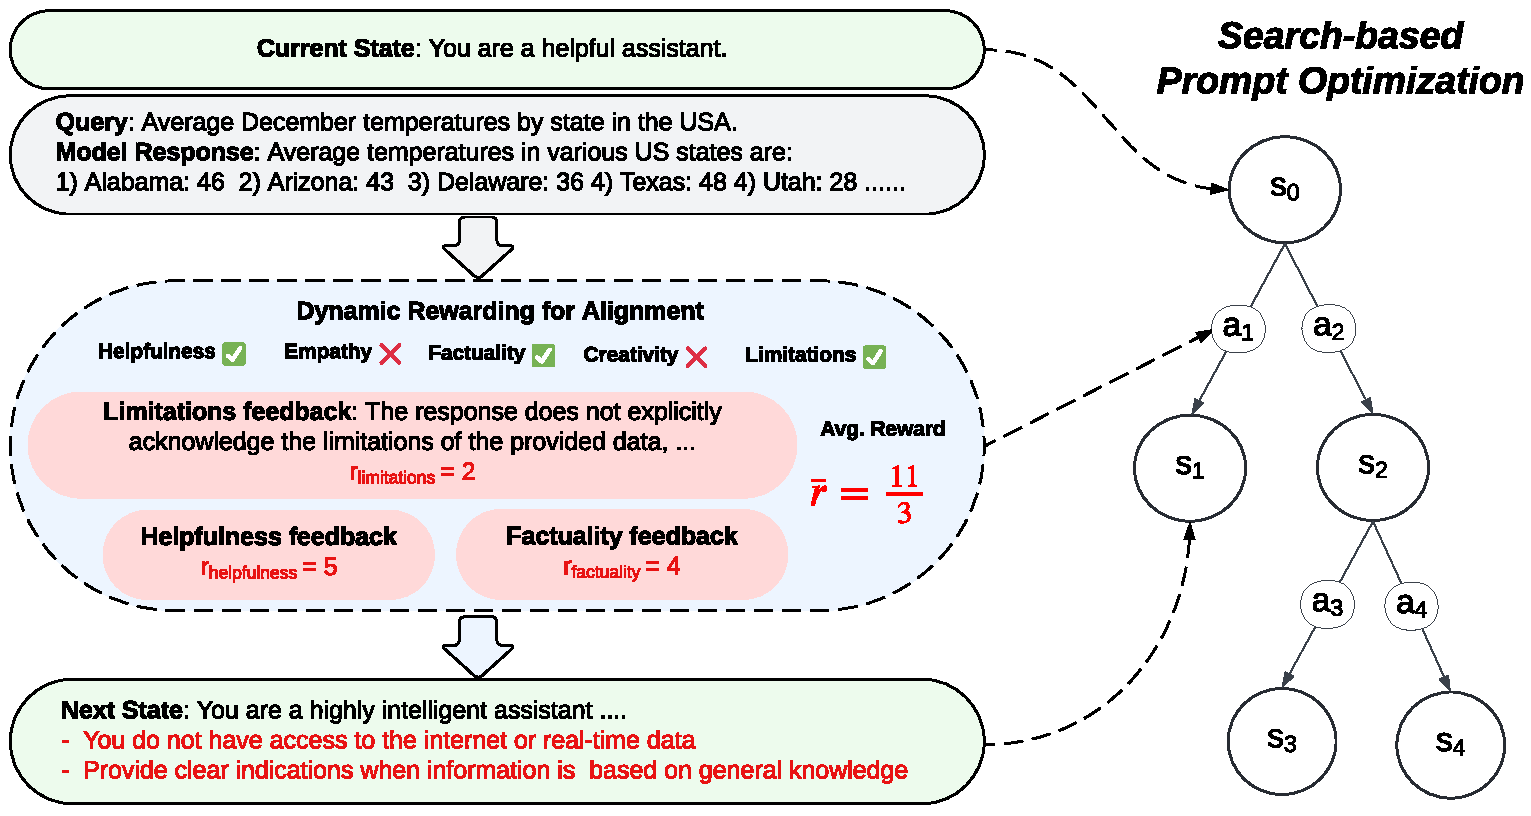
\includegraphics[width=0.95\linewidth]{images/Dynamic_Rewarding.pdf}
    \vspace{-8pt}
    \caption{带有提示优化的动态奖励整体框架(\ours)。该优化问题被建模为一个马尔可夫决策过程(MDP),并通过束搜索(beam search)求解以优化对齐提示。动态奖励作为该框架中集成的一项新技术,允许灵活分配奖励,以检测并解决当前大语言模型中的对齐弱点,从而增强整体优化过程。}
    \label{fig:dynamic_rewarding}
    \vspace{-15pt}
\end{figure*}

\noindent \textbf{免微调对齐(Tuning-Free Alignment).}
近年来,对齐研究的一个新趋势是无需更新参数来对齐大语言模型,通常作为训练后的处理步骤。当前主要有两类研究方向。第一类方法使用精心策划的人类标注和ICL示例进行模型对齐~\cite{han2023context, Lin2024ReAlign, zhao2024context};第二类方法则采用基于解码的策略,通过对齐奖励引导生成的token及其搜索过程~\cite{li2023rain, khanov2024args, huang2024deal}。虽然这些方法无需微调,第一类仍需人类策划,并且通常性能不及经过SFT/RLHF微调的模型;第二类虽然效果较好,但每次查询的推理成本较高,计算代价昂贵。值得一提的是,另一个有前景的方向是通过表示工程进行成本高效的对齐~\cite{zou2023representation, wu2024reft},该方法试图通过调整大语言模型的表示向量来实现对齐~\cite{li2024inference, kong2024aligning, wang2024inferaligner}。然而,这些方法并非真正意义上的免微调,通常仍需额外数据或模型训练来识别嵌入空间中的对齐方向。相比之下,\ours 无需任何额外标注或模型训练,仅需对每个模型进行一次性优化即可在性能上超过SFT/RLHF微调模型。

\noindent \textbf{提示优化(Prompt Optimization).}
发现最优的离散提示在当下变得尤为重要。现代大语言模型的提示通常分为两部分:上下文学习示例和详细指令。前者通常被视为一个检索问题,通过各种方案选择具有影响力的示例~\cite{rubin2021learning, dong2022survey}。而对后者的优化近来成为研究重点,通常被建模为一个采样或搜索问题。一般来说,会先提供一个初始提示(例如一个基本提示,“You are a helpful assistant”),然后启动一个迭代过程,在每一轮生成多样的提示候选,并保留最佳候选用于下一轮。为增加提示候选的多样性,研究提出了多种采样策略,例如反向翻译~\cite{xu2022gps}、进化操作~\cite{fernando2023promptbreeder}、自我批判~\cite{wang2023promptagent}。同时,也有多种搜索框架被提出,如蒙特卡洛搜索~\cite{zhou2022large}、进化算法~\cite{fernando2023promptbreeder, yang2023large}、束搜索~\cite{pryzant2023automatic}、以及蒙特卡洛树搜索(MCTS)~\cite{wang2023promptagent}。\ours 基于近年来的搜索优化方法,并引入动态奖励等新技术,有效应对对齐问题。
